\documentclass[10pt, a4paper]{article}

\usepackage[english]{babel}
\usepackage[utf8]{inputenc}
\usepackage{float}
\usepackage[]{amsmath} 
\usepackage{graphicx}

% Define question and answer command
\newcounter{qcounter}
\newcommand{\q}[2]
{
    \textbf{Task \refstepcounter{qcounter} \arabic{qcounter}: #1} \\
    #2
    \par
    \vspace{0.5cm}
} 

\begin{document}

\begin{titlepage}
\centering
{
 \scshape \LARGE 
EL2450 Homework 2
}
\vfill
Andreas Fr\"{o}derberg - 19880730-7577
\par
Martin Favre - 19920130-0010
\end{titlepage}

\section{Rate Monotonic scheduling}
\label{sec:rate_monotonic_scheduling}

\q %1
{
    Explain what Rate Monotonic scheduling means.
}
{
    Rate Monotonic scheduling means that all tasks are given a priority. At te
    beginning of each cycle, the task with the highest priority is run until
    Rate Monotonic scheduling means that all tasks are given a priority. At te
    beginning of each cycle, the task with the highest priority is run until
    completion.
}

\q %2
{
	Are the three tasks schedulable?
}
{
	Calculating the utilization factor U from 
	\begin{equation}
		U = \sum\limits_{i=1}^n \frac{C_i}{T_i}=\frac{6}{20} + \frac{6}{29} +
        \frac{6}{35} = 0.75
	\end{equation}	
	The rules states that if $U<1$ the set is schedulable.
}
\q %3
{
    What are the differences in control performance between the different
    pendulums?
}
{
    All pendulums are asymptotically stable and have similar control
    performance. The performance is shown in Figure~\ref{fig:T3_dmperformance}.
    \begin{figure}[H]
        \centering
        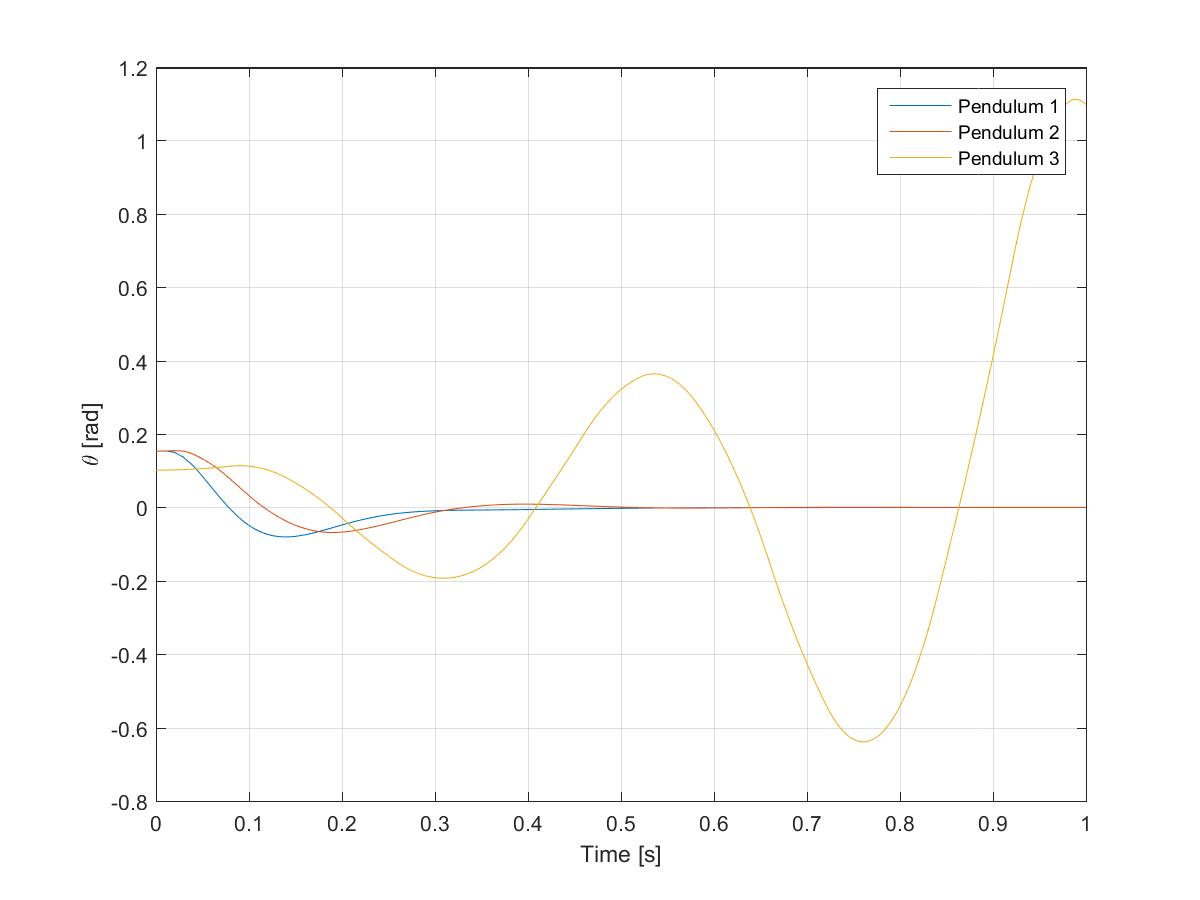
\includegraphics[width=1\linewidth]{../Matlab/HW2_sources_Windows64bit/images/Task_3_dm_performance.png}
        \caption{Performance of pendulums under rate monotonic scheduling.}
        \label{fig:T3_dmperformance}
    \end{figure}
}
\q %4
{
    Compare against the schedule in the model. Does it match?
}
{
    As can be seen below in Figure~\ref{fig:Task_4_sch_6ms}, the schedules
    match. The tasks are schedulable as stated in q2.
    \begin{figure}[H]
        \centering
        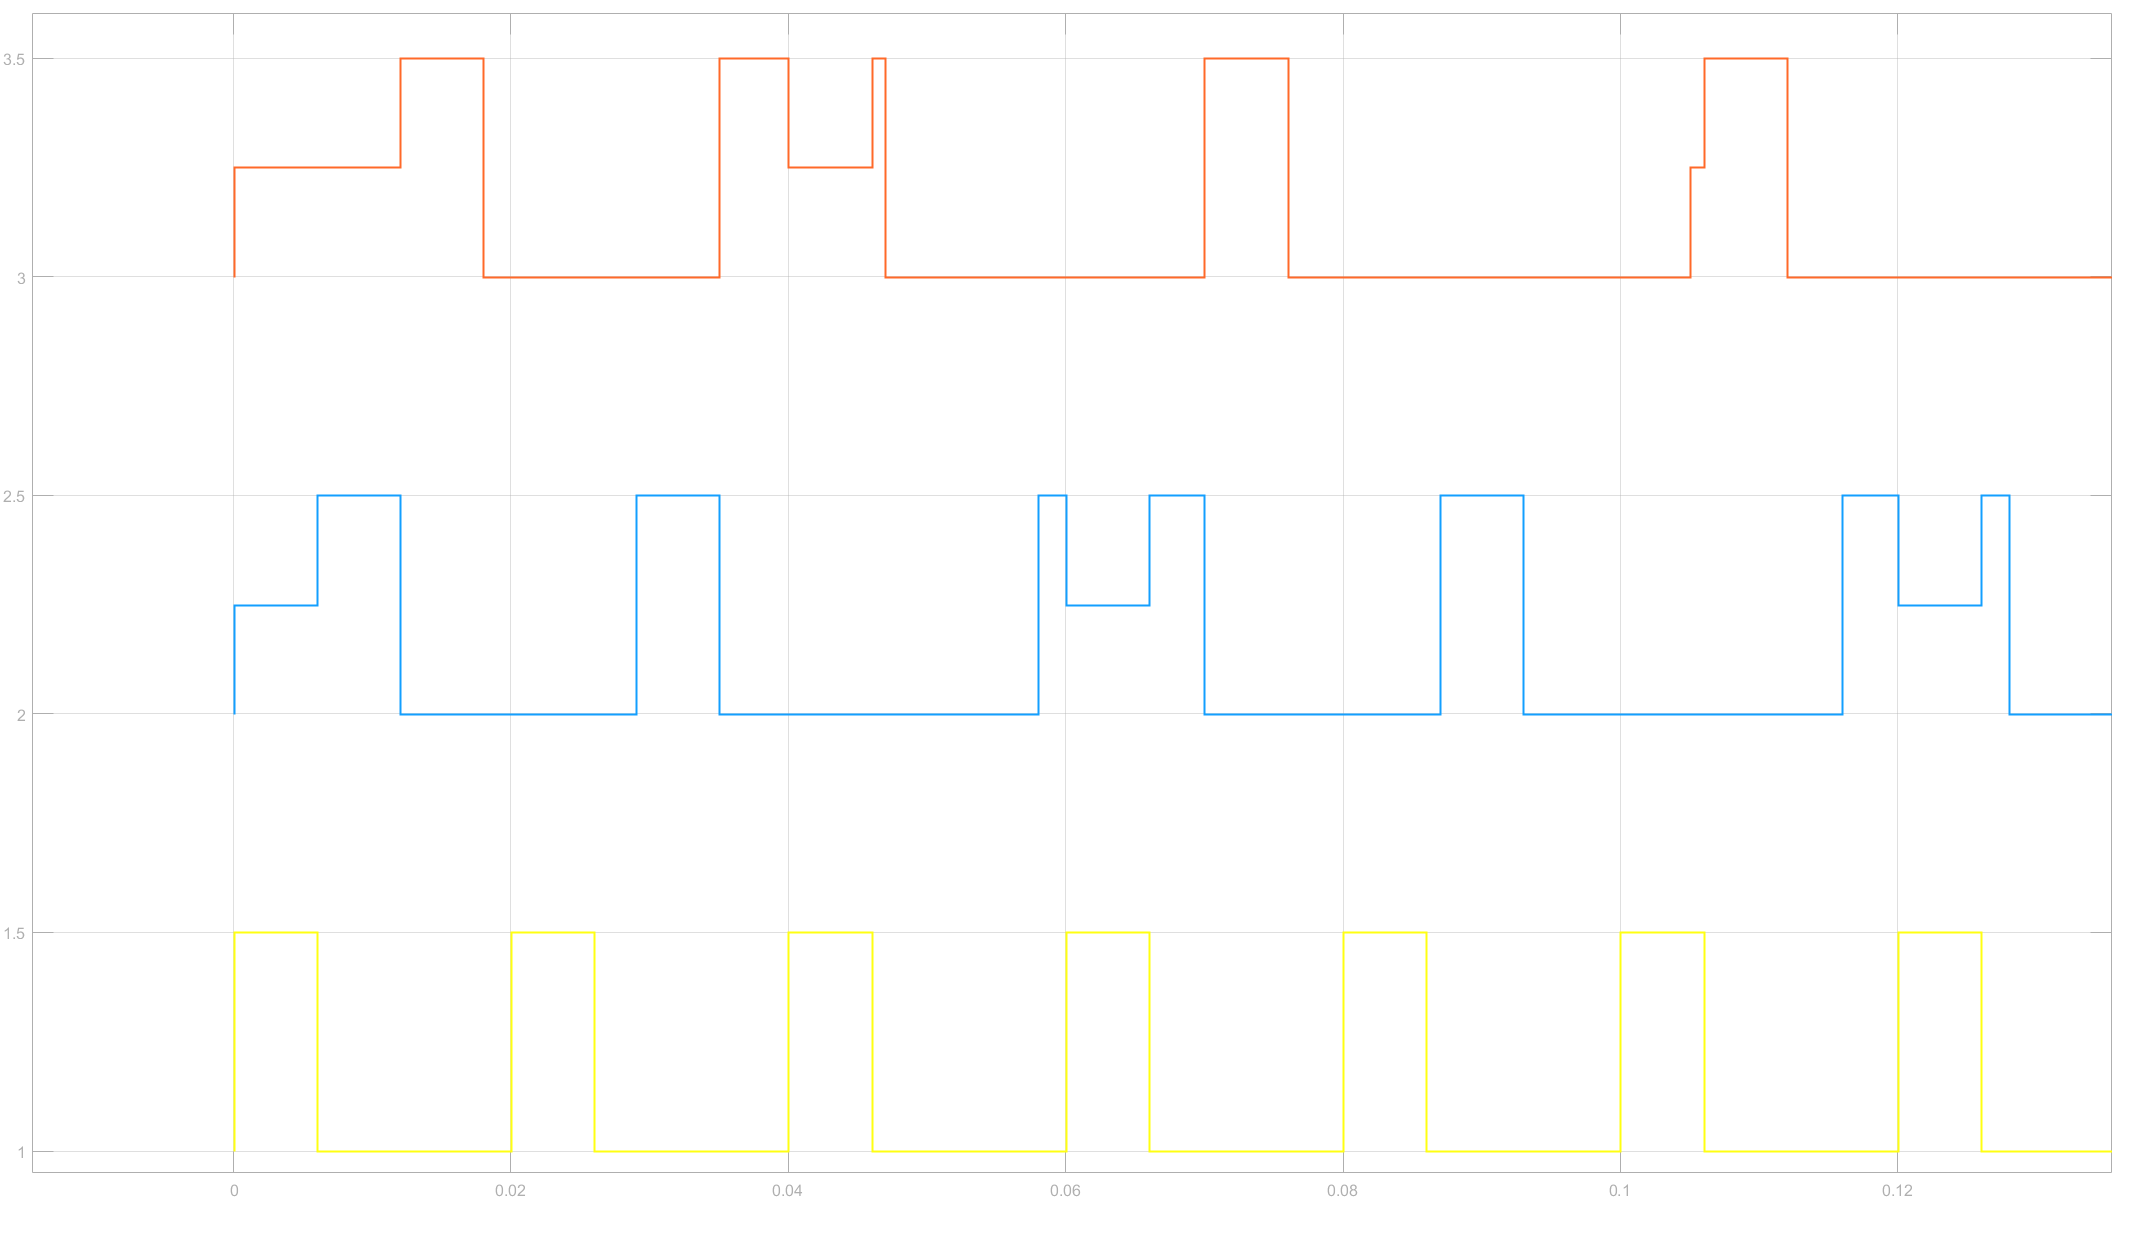
\includegraphics[width=1\linewidth]{../Matlab/HW2_sources_Windows64bit/images/Task_4_sch_6ms.png}
        \caption{Schedule for pendulums when computation time of all is 6 ms.
        Yellow is small pendulum, blue is medium and red is big.}
        \label{fig:Task_4_sch_6ms}
    \end{figure}
}
    
    

\end{document}
